\documentclass[12pt]{article}
\usepackage{graphicx}
\usepackage[a4paper, total={7in, 9in}]{geometry}
\usepackage{titlesec}
\graphicspath{ {images/} }

\titleformat{\paragraph}
{\normalfont\normalsize\bfseries}{\theparagraph}{1em}{}
\titlespacing*{\paragraph}
{0pt}{3.25ex plus 1ex minus .2ex}{1.5ex plus .2ex}

\title{DMT - Homework 1}
\author{
        Tran Luong Bang, Juan Mata Naranjo \\
                Master in Data Science}
\date{\today}

\begin{document}
\maketitle
\newpage

\section{Part 1.1}

Before we deep dive into each of the individual datasets and their respective results we will start out by first giving a brief overview of the number of documents we have, the number of queries applied over these documents and finally the number of queries for which we have their ground truth at our disposal. We will see that the number of ground truth results we have are much less than the total number of queries. For the evaluation metrics we will assume that the queries for which we don't have ground truth don't exist (we remove them from all evaluation metrics). We will then also outline the different text-analyzer $+$ scoring-functions we have deployed.

\begin{table}[]
\centering
\begin{tabular}{|l|l|l|}
\hline
                  & Cranfield Dataset & Time Dataset \\ \hline
Num Indexed Docs  & 1400                 & 423            \\ \hline
Num Queries       & 225                 & 83            \\ \hline
Num Queries in GT & 110                 &  80           \\ \hline
\end{tabular}
\caption{Overview Table}
\label{Overview Table}
\end{table}

\begin{table}[]
\centering
\resizebox{\textwidth}{!}{%
\begin{tabular}{|p{1cm}|p{10cm}|p{10cm}|}
\hline
\textbf{Conf ID} &
  \textbf{Text Analyzer} &
  \textbf{Scoring Functions} \\ \hline
1 &
  RegexTokenizer() $|$ LowercaseFilter() $|$ StopFilter(stoplist = STOP\_WORDS) &
  scoring.MultiWeighting(scoring.Frequency(), title=scoring.BM25F(), content=scoring.TF\_IDF()) \\ \hline
2 &
  RegexTokenizer()$|$ StopFilter(stoplist = STOP\_WORDS)$|$ LowercaseFilter() $|$ StemFilter() &
  scoring.BM25F(K1=1.2, B=.75) \\ \hline
3 &
  StemmingAnalyzer(stoplist=STOP\_WORDS) &
  scoring.TF\_IDF() \\ \hline
4 &
  FancyAnalyzer() &
  scoring.BM25F(K1=2, B=.8) \\ \hline
5 &
  SimpleAnalyzer() &
  scoring.TF\_IDF() \\ \hline
6 &
  StandardAnalyzer() &
  scoring.Frequency() \\ \hline
7 &
  FancyAnalyzer() &
  scoring.MultiWeighting(scoring.Frequency(), title=scoring.TF\_IDF(), content=scoring.BM25F()) \\ \hline
8 &
  StemmingAnalyzer(stoplist=STOP\_WORDS) &
  scoring.BM25F() \\ \hline
9 &
  RegexTokenizer()$|$ StopFilter(stoplist = STOP\_WORDS)$|$ LowercaseFilter() $|$ StemFilter() &
  scoring.MultiWeighting(scoring.Frequency(), title=scoring.TF\_IDF(), content=scoring.BM25F(K1=2, B=.8)) \\ \hline
10 &
  SimpleAnalyzer() &
  scoring.BM25F(K1=1.2, B=.75) \\ \hline
11 &
  StemmingAnalyzer(stoplist=STOP\_WORDS) &
  scoring.BM25F(K1=2, B=.8) \\ \hline
12 &
  FancyAnalyzer() &
  scoring.TF\_IDF() \\ \hline
\end{tabular}}
\caption{Configuration Overview}
\label{tab:my-table}
\end{table}


\subsection{Cranfield Dataset:}

We will now continue by presenting the most relevant results on the Cranfield Dataset. The first result presented is a table containing all the configurations (ordered by the MRR evaluation metric from highest to lowest), and the R-Precision metrics:

\begin{table}[]
\centering
\begin{tabular}{|c|c|c|c|c|c|c|c|}
\hline
\multicolumn{1}{|l|}{\textbf{Conf ID}} &
  \multicolumn{1}{l|}{\textbf{MRR}} &
  \multicolumn{1}{l|}{\textbf{Mean}} &
  \multicolumn{1}{l|}{\textbf{Min}} &
  \multicolumn{1}{l|}{\textbf{1st quartile}} &
  \multicolumn{1}{l|}{\textbf{Median}} &
  \multicolumn{1}{l|}{\textbf{3rd quartile}} &
  \multicolumn{1}{l|}{\textbf{Max}} \\ \hline
11 & 0.527 & 0.273 & 0 & 0 & 0.250 & 0.429 & 1.000 \\ \hline
2  & 0.522 & 0.278 & 0 & 0 & 0.250 & 0.490 & 1.000 \\ \hline
8  & 0.522 & 0.278 & 0 & 0 & 0.250 & 0.490 & 1.000 \\ \hline
7  & 0.504 & 0.255 & 0 & 0 & 0.250 & 0.460 & 0.667 \\ \hline
9  & 0.499 & 0.260 & 0 & 0 & 0.250 & 0.500 & 1.000 \\ \hline
4  & 0.496 & 0.264 & 0 & 0 & 0.250 & 0.448 & 1.000 \\ \hline
10 & 0.475 & 0.245 & 0 & 0 & 0.250 & 0.429 & 0.667 \\ \hline
3  & 0.416 & 0.178 & 0 & 0 & 0.143 & 0.296 & 1.000 \\ \hline
12 & 0.388 & 0.177 & 0 & 0 & 0.143 & 0.286 & 1.000 \\ \hline
1  & 0.384 & 0.184 & 0 & 0 & 0.143 & 0.286 & 1.000 \\ \hline
6  & 0.303 & 0.131 & 0 & 0 & 0.000 & 0.217 & 1.000 \\ \hline
5  & 0.166 & 0.074 & 0 & 0 & 0.000 & 0.103 & 0.833 \\ \hline
\end{tabular}
\caption{MRR and R-Precision Overview}
\label{MRR}
\end{table}




\begin{center}
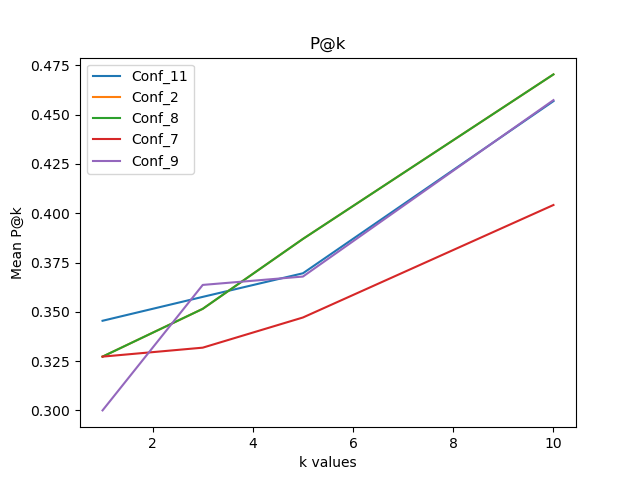
\includegraphics[scale=.75]{Pk.png}
\end{center}


\begin{center}
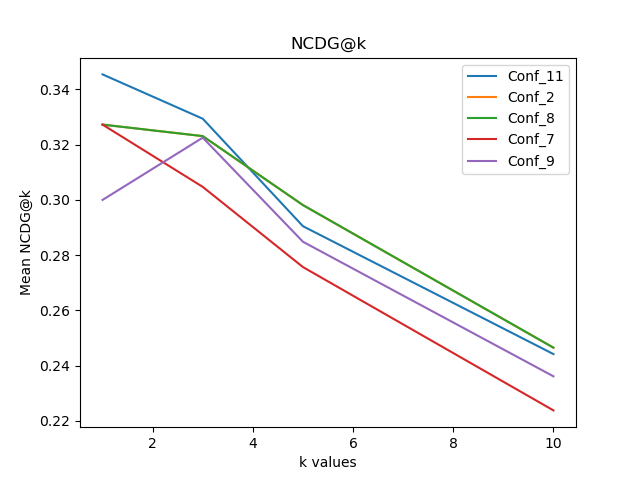
\includegraphics[scale=.75]{NCDGk.png}
\end{center}


\subsection{Time Dataset:}


\section{Part 2.1}

The first thing we have to do before running the LSH algorithm is to figure out the best $r$ (number of rows in each band), $b$ (number of bands) and $n$ (number of hash functions used) parameters such that we can minimize the number of False Positives and False Negatives. In particular, the choice of parameters will mainly help us to minimize the quantity of False Negatives. Taking inot account the other constraints which are the following:

\begin{equation}
r \cdot b = n
\end{equation}


\begin{equation}
0.97 > 1 - (1-0.95^r)^b
\end{equation}

From the second constraint we can see that the following relation holds:

\begin{equation}
b > \frac{log(1-0.97)}{log(1-0.95^r)}
\end{equation}

In order to minimze the False Negatives we will stress the $0.97$ boud as much as possible, specifically up to $0.999$. This will reduce the number of False Negatives, but will of course increase the number of False Positives. Since we will be able to remove some of the False Positives later on we will not worry too much for the moment. With this assumption, fixing a value of $r=15$ we have decided to use the following parameters:

\begin{table}[]
\centering
\begin{tabular}{|l|l|}
\hline
\textbf{r} & 15    \\ \hline
\textbf{b} & 12   \\ \hline
\textbf{n} & 180 \\ \hline
\end{tabular}
\caption{Parameter Overview}
\label{tab:my-table}
\end{table}

\begin{center}
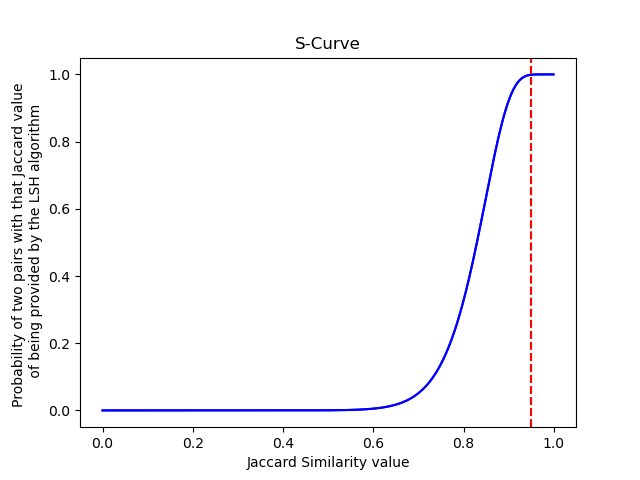
\includegraphics[scale=.75]{Splot.png}
\end{center}

After running the LSH algorithm with the previous set of parameters we got the following number of \textit{potential} near duplicate matches: \textbf{34655}. However, as we already mentioned before, we can still reduce the number of False Positives a posteriori by computing the Jaccard Similarity over the set of pairs provided by the LSH tool, and therefore eliminating those pairs which we will not consider as near duplicates. For this purpose we have used the code named "False Positive Reduction" (in which we re-compute the real Jaccard similarity and not the approximated one), after which the number of \textit{final} near duplicates was: \textbf{33868}. Of course, in this specific case we could reduce the number of  False Negatives, making the LSH algorithm return more potential pairs (approx. 13$\%$). This might be too many potential pairs in other applications where instead of 250K documents we have billion documents. In these cases the percentage of potential pairs in output must be much lower, and therefore we might have to deal with having more False Negatives.

The total time required to run the LSH tool with the parameters highlighted previously was of \textbf{7 minutes and 15 seconds} on our machine.


\end{document}